% -------------------------------------------------------------------------------------
% Einlesen der .sty-Dateien
% -------------------------------------------------------------------------------------
%  se-pa1-input-styles.tex
%
%  Joerg Baumgart 01.08.2011
%
%  Zusammenfassung und Konfiguration wichtiger Styles f\"ur die 
%  Erzeugung von Seminar-, Projekt- und Bachelorarbeiten
%
%
\documentclass[12pt,BCOR=10mm,headinclude=on,footinclude=off,bibliography=totoc]{scrreprt}
\usepackage[T1]{fontenc}
\usepackage[utf8]{inputenc}
\usepackage[ngerman]{babel} % Deutsche Einstellungen
\usepackage{lmodern}

\usepackage{tikz} % Graphikpaket, das zu pdfLaTeX kompatibel ist
\usepackage{xkeyval} % Definition von Kommandos mit mehreren optionalen Argumenten
\usepackage{listings} % Formatierung von Programmlistings
\usepackage{graphicx} % Einbinden von Graphiken
\usepackage{ifthen}
\usepackage{color}
\usepackage{slashbox} % Diagonalen in Tabellenfeldern
\usepackage{framed} % Erzeugung schwarzer Linien am linken Rand zur Hervorhebung von Textteilen
\usepackage{caption} % Korrektes Setzen einer mehrzeiligen float-Unterschrift bei neu definierten float-Umgebungen
%\usepackage{floatrow}

% Es wird jeweils die sty-Datei importiert und entsprechende Konfigurationseinstellungen werden vorgenommen
%
\usepackage{sty/se-jb-scrpage2} % Formatierung der Kopf- und Fu{\ss}zeilen
\usepackage{sty/se-jb-footmisc}    % Fussnoten besser formatieren

\usepackage{sty/se-jb-glossaries} % Abk\"urzungsverzeichnis, Symbolverzeichnis, Glossar
   
\usepackage{sty/se-jb-floatrow}    % Definition und Konfiguration von float-Umgebungen (figure, table, die neue programm-Umgebung)
% Achtung: se-jb-varioref muss nach se-jb-floatrow importiert werden; 
% andernfalls ist der counter programm f\"ur die labelformat-Anweisung noch nicht definiert   
\usepackage{sty/se-jb-varioref}   % Definition von Querverweisen
\usepackage{sty/se-jb-chngcntr}   % Kapitelweise oder globale Nummerierung von Abbildungen etc.
   
\usepackage{sty/se-jb-listen} % Definition neuer, besser formatierter Listen
\usepackage{sty/se-jb-wa-kommandos} % neue Kommandos f\"ur Seminar-, Projekt- und Bachelorarbeiten


% -------------------------------------------------------------------------------------
% Individuelle Konfiguration des Dokumentes
% -------------------------------------------------------------------------------------
%  Individuelle Konfiguration einer Projektarbeit
%
%
%
%

%
% Literaturverzeichnis
% 
%\usepackage{se-jb-jurabib-theisen} % Literaturverzeichnis gem\"ass den Vorgaben von Theisen aufbauen

\usepackage{bibgerm}
\usepackage{url}
\usepackage{booktabs}
\usepackage{array}

\providecommand{\seCite}[3]{\ifthenelse{\equal{#2}{}}{#1 \cite{#3}}{#1 \cite[#2]{#3}}}


\providecommand{\seFootcite}[3]{\ifthenelse{\equal{#2}{}}{\footnote{#1 \cite{#3}}}{\footnote{#1 \cite[#2]{#3}}}}


% Weitere Optionseinstellungen f\"ur das Koma-Script
%
% Zwischen Abs\"atzen einen Abstand von 0.5 \baselineskip erzeugen
\KOMAoption{parskip}{full}
%
% Vergleiche Duden "Gliederung von Nummern, S.111" 
% DIN 5008 anschauen, wenn sie neu ver\"offentlicht wurde
\KOMAoption{numbers}{noendperiod}
%
%



%  Voreinstellungen f\"ur floats
%  Durch die verwendeten Parameter wird die Wahrscheinlichkeit deutlich kleiner, 
%  dass Gleitobjekte (z. B. Abbildungen) ans Ende des Dokumentes verschoben 
%  werden; 
%  Achtung: clearpage erzwingt die Ausgabe von Gleitobjekten
%
\renewcommand{\topfraction}{1}  % Gleitobjekte d\"urfen eine Seite zu 100% belegen 
\renewcommand{\bottomfraction}{1} % Entsprechender Wert f\"ur den unteren Teil der Seite
\renewcommand{\textfraction}{0} % Eine Seite darf auch ohne Fliesstext existieren
%%%\renewcommand{\floatpagefraction}{1} % Bedeutung unklar, daher keine Ver\"anderung des Vorgabewertes 
                                                                        % von 0.5; eventuell bringt ein \"Anderung auf 1 etwas, wenn 
                                                                         % Probleme mit floats auftreten
                                                                         
                                                                         
                                                                         
% Konfiguration von Programm-Listings
% 
% Achtung: hier gibt es nahezu beliebig viele weitere Konfigurationm\"oglichkeiten; vgl. Paketdokumentation
%
\lstset{language=[R/3 6.10]ABAP,basicstyle=\ttfamily,keywordstyle=\color{blue},captionpos=b,aboveskip=0mm,belowskip=0mm,
          xleftmargin=0em}        
          
%
% Grundkonfiguration der Abs\"ande zwischen den Items der maximal f\"unf Verschachtelungsebenen der 
% neuen Listenumgebungen
%                                                                             
% Initialisierung der Abst\"ande zwischen den items f\"ur seList; Grundeinheit: 0.5\baselineskip; siehe se-jb-listen
\seSetlistbaselineskip{1}{0.75}{0.75}{0.75}{0.75}
% Initialisierung der Abst\"ande zwischen den items f\"ur seToplist; Grundeinheit: 0.5\baselineskip; siehe se-jb-listen
\seSettoplistbaselineskip{1}{0.75}{0.75}{0.75}{0.75}     


%
%  Konfiguration der verschiedenen Verzeichnisse
%
%  abstandEintrag: Wert wird mit \baselineskip multipliziert
%

%
%  Abbildungsverzeichnis
%
\seKonfigurationAbb[
%verzeichnisname=Abbildungsverzeichnis,
labeltextLinks=, % kein Text links;
%labeltextRechts=:,
labelbreite=1cm,
%labeleinzug=1cm,
%abstandEintrag=1,
newpage=ja,
%pnumwidth=20mm,
%dotsep=1000,
%tocrmarg=4.5cm,
%abstandVerzeichnis=-1mm
]

%
% LIstingverzeichnis
%
\seKonfigurationPrg[
%verzeichnisname=Listing-Verzeichnis,
labeltextLinks=,
%labeltextRechts=:,
labelbreite=1cm,
%labeleinzug=2cm,
%abstandEintrag=1,
newpage=ja,
%%pnumwidth=20mm,
%dotsep=1000,
%tocrmarg=4.5cm,
%abstandVerzeichnis=-10mm
]

%
% Tabellenverzeichnis
%
\seKonfigurationTab[
%verzeichnisname=Liste der Tabellen,
labeltextLinks=,
%labeltextRechts=:,
labelbreite=1cm,
%labeleinzug=0.5cm,
%abstandEintrag=1,
newpage=ja,
%pnumwidth=20mm,
%dotsep=1000,
%tocrmarg=4.5cm,
%abstandVerzeichnis=-10mm
]

%
% Abk\"urzungsverzeichnis
%
\seKonfigurationAbk[
%verzeichnisname=Liste der Abk\"urzungen,
%labelbreite=3cm,
%labeleinzug=0.5cm,
%abstandEintrag=1,
%newpage=ja,
%abstandVerzeichnis=-10mm
]

%
% Symbolverzeichnis
% 
\seKonfigurationSym[
%verzeichnisname=Liste der Symbole,
%labelbreite=4cm,
%labeleinzug=3.5cm,
%abstandEintrag=1,
newpage=ja,
%abstandVerzeichnis=-10mm
]

%
% Glossar
%
\seKonfigurationGlo[
%verzeichnisname=Glossar,
%abstandEintrag=0,
]



% (eventuelle) Neudefinition f\"ur die Unter-/\"Uberschriften von Abbildungen, Tabellen und Listings
%
%
%\renewcommand{\seCaptionNameAbbildung}{Abb.}
%\renewcommand{\seCaptionNameTabelle}{Tab.}
%\renewcommand{\seCaptionNameProgramm}{Prg.}


% % (eventuelle) Neudefinition f\"ur Querverweise innerhalb des Textes
%
%
%
%\renewcommand{\seQuerverweisSeite}{Seite}
%\renewcommand{\seQuerverweisAbbildung}{Abb.}
%\renewcommand{\seQuerverweisTabelle}{Tab.}
%\renewcommand{\seQuerverweisProgramm}{Prg.}
%\renewcommand{\seQuerverweisKapitel}{Kap.}
%\renewcommand{\seQuerverweisGleichung}{Gl.}

% Kommandos, die direkt nach \begin{document} ausgef\"uhrt werden m\"ussen
%
%
%
\AtBeginDocument{%
\renewcommand{\listfigurename}{\seAbbildungenVerzeichnisname}
\renewcommand{\listtablename}{\seTabellenVerzeichnisname}
\renewcommand{\figurename}{\seCaptionNameAbbildung}
\renewcommand{\tablename}{\seCaptionNameTabelle}
\pagenumbering{roman}
}
                                                              
                                                                         

% -------------------------------------------------------------------------------------
% Individuelle Definition von Abk\"urzungen, Symbolen und eventuell Glossareintr\"agen
% -------------------------------------------------------------------------------------
%--------------------------------------------------------------------------------------
% Trennungsregeln
%--------------------------------------------------------------------------------------
\hyphenation{prob-lem-los}
\hyphenation{Inter-banken-han-del}
\hyphenation{Business-Objects}
\hyphenation{Web-ser-vice}
\hyphenation{Web-ser-vi-ces}
\hyphenation{Dash-board}
\hyphenation{Dash-boards}
\hyphenation{Zu-gangs-be-schrän-kung-en}
\hyphenation{ge-star-tet}
\hyphenation{NSFR}
\hyphenation{LCR}
\hyphenation{Va-ri-a-blen-aus-prä-gung-en}
\hyphenation{Dia-gramm}
\hyphenation{An-wen-dung}
\hyphenation{An-wen-dung-en}
\hyphenation{An-for-de-rung}
\hyphenation{An-for-de-rung-en}
\hyphenation{Haupt-an-for-de-rung-en}
\hyphenation{tech-nisch-en}
\hyphenation{Funk-ti-o-na-li-tät}
\hyphenation{Or-ches-trie-rung}
\hyphenation{Xcel-si-us}
\hyphenation{Xcel-si-us-A-dap-ter}
\hyphenation{Ein-stel-lung}
\hyphenation{Ein-stel-lung-en}
\hyphenation{Li-qui-di-tät}
\hyphenation{Li-qui-di-täts-ri-si-ko}
\hyphenation{Li-qui-di-täts-ri-si-ko-ma-nage-ment}
\hyphenation{Dash-board}


%--------------------------------------------------------------------------------------
% Abkürzungen
%--------------------------------------------------------------------------------------
\newacronym{dbms}{DBMS}{Da\-ten\-bank\-ma\-nage\-ment\-sys\-tem}
\newacronym{sql}{SQL}{Structured Query Language}
\newacronym{MaRisk}{MaRisk}{Mindestanforderungen an das Risikomanagement}
\newacronym{LiqV}{LiqV}{Liquiditätsverordnung}
\newacronym{ngap}{NGAP}{Next Generation ABAP Plattform}
\newacronym{erp}{ERP}{Enterprise Resource Planning}
\newacronym{crm}{CRM}{Customer Relationship Management}
\newacronym{saplrm}{SAP\,\,LRM}{SAP Liquidity Risk Management}
\newacronym{http}{HTTP}{Hypertext Transfer Protocol}
\newacronym{xml}{XML}{Extensible Markup Language}
\newacronym{NetWeaver}{NetWeaver}{SAP NetWeaver Application Server}
\newacronym{xcelsius}{Xcelsius}{BusinessObjects Xcelsius}
\newacronym{biz}{BIZ}{Bank für Internationalen Zahlungsausgleich}
\newacronym{url}{URL}{Uniform Resource Locator}
\newacronym{wysiwyg}{WYSIWYG}{What You See Is What You Get}
\newacronym{sdk}{SDK}{Software Development Kit}
\newacronym{lcr}{LCR}{Liquidity Coverage Ratio}
\newacronym{nsfr}{NSFR}{Net Stable Funding Ratio}
\newacronym{rest}{REST}{Representational State Transfer}
\newacronym{ria}{RIA}{Rich Internet Application}
\newacronym{abap}{ABAP}{Advanced Business Application Programming}
\newacronym{bw}{BW}{Business Warehouse}
\newacronym{libor}{LIBOR}{London Inter Bank Offered Rate}

%--------------------------------------------------------------------------------------
% Glossareinträge
%--------------------------------------------------------------------------------------

\newglossaryentry{glos:netFramework}{
first=.NET Framework\textsuperscript{GL},
name=.NET Framework,
description={ Das .NET Framework ist eine Plattform von Microsoft, mit der Anwendungen für das Betriebssystem Microsoft Windows erstellt und ausgeführt werden können. Die wichtigsten Komponenten sind Klassenbibliotheken, zum Beispiel für die Entwicklung der Oberflächen, und die Common Language Runtime. Die Anwendungen können in verschiedenen Programmiersprachen geschrieben werden. Zu den unterstützten Sprachen zählen unter anderem C++ und C\#. Der Quellcode wird dann in die Common Intermediate Language compiliert. Diese Zwischensprache kann dann von der Common Language Runtime ausgeführt werden.\seFootcite{vgl.}{S.382ff}{Lou.10}}
}


\newglossaryentry{glos:interbankenhandel}{
first=Inter\-banken\-han\-del\textsuperscript{GL},
name=Interbankenhandel,
description={Der Interbankenhandel ist der Handel von Wertpapieren, Anlagen oder ähnlichem zwischen Banken. Synonym wird auch oft der Begriff Interbankenmarkt verwendet. Für die Zinssätze, mit denen Banken untereinander handeln, existieren anerkannte Referenzen, wie zum Beispiel die \gls{libor}. In Liquiditätsengpässen kann der Interbankenhandel eine wichtige Refinanzierungsrolle darstellen. Der Handel zwischen Banken hängt sehr stark von dem gegenseitigen Vertrauen ab.\seFootcite{vgl.}{S.145f}{Wil.10}}
}

\newglossaryentry{glos:bankrun}{
first=Bankenpanik\textsuperscript{GL},
name=Bankenpanik,
description={Eine Bankenpanik ist ein Ereignis, bei dem eine große Anzahl von Anlegern versucht, ihre Einlagen bei einer Bank abzuziehen. Der Grund kann zum einen in der Veröffentlichung von schlechten Ergebnissen der Bank und damit in einem Vertrauensverlust begründet sein, zum anderen aber auch rein spekulativ sein. Für die Bank besteht die Gefahr der Insolvenz. Im Englischen spricht man von einem Bank Run.\seFootcite{vgl.}{S.1f}{Sch.11}}
}

\newglossaryentry{glos:sqlscript}{
first=SQLScript\textsuperscript{GL},
name=SQLScript,
description={SQLScript ist eine Erweiterung der Abfragesprache SQL und wird in der Datenbank von SAP HANA verwendet. Mit Hilfe von SQLScript lässt sich Anwendungslogik in die Datenbank auslagern. Dazu wurden unter anderem Datentypen, Prozeduren und Kontrollstrukturen hinzugefügt.\seFootcite{vgl.}{S.9f}{SQLScript.11}}
}

\newglossaryentry{glos:ria}{
first=\gls{ria}\textsuperscript{GL},
name=\gls{ria},
sort=RIA,
description={Unter dem Begriff Rich Internet Application werden Webanwendungen bezeichnet, die in ihrer Funktionalität und ihrem Aussehen Desktopanwendungen ähneln. Erstmals eingeführt wurde der Begriff von Macromedia. Zwischen normalen Webanwendungen und RIA kann keine klare Grenze gezogen werden. Ein wichtiges Indiz für eine RIA ist der Einsatz von Technologien wie zum Beispiel Adobe Flash, Adobe Air oder Microsoft Silverlight.\footnote{\seCite{vgl.}{S.32f}{DD.08} \seCite{und}{S.3f}{Pfe.09}\newline
Adobe Flash - http://www.adobe.com/products/flashplayer.html \newline
Adobe Air - http://www.adobe.com/products/air.html \newline
Microsoft Silverlight - http://www.microsoft.com/silverlight/} }
}

\newglossaryentry{glos:bydesign}{
first=SAP Business ByDesign\textsuperscript{GL},
name=SAP Business ByDesign,
description={SAP Business ByDesign ist eine Anwendung von SAP für mittelständige Unternehmen. Zu dem Funktionsunfang gehört sowohl ein \gls{erp}- als auch eine \gls{crm}-Lösung. Die Besonderheit von SAP Business ByDesign ist, dass es auf Servern bei SAP betrieben wird und Kunden die Anwendung mieten und über das Internet konsumieren.}
}

\newglossaryentry{glos:lcr}{
first=\gls{lcr}\textsuperscript{GL},
name=\gls{lcr},
sort=LCR,
description={
Die \gls{lcr}, die auch als Mindestliquiditätsquote bezeichnet wird, ist eine requlatorische Vorgabe im Rahmen von Basel III. Durch die Einhaltung soll sichergestellt werden, dass eine Bank unerwartete Zahlungsmittelabflüsse über einen Zeitraum von 30 Tagen mit eigenen liquiden Aktiva ausgleichen kann.\seFootcite{vgl.}{S.4}{BIS.10}
}
}

\newglossaryentry{glos:nsfr}{
first=\gls{nsfr}\textsuperscript{GL},
name=\gls{nsfr},
sort=NSFR,
description={
Die \gls{nsfr} ist eine requlatorische Vorgabe im Rahmen von Basel III und soll eine mittel- und langfristige Refinanzierung von Banken fördern. Er besteht aus dem Verhältnis von verfügbaren und erforderlichen langfristiger Refinanzierung. Sie wird auch als strukturelle Liquiditätsquote beizeichnet.\seFootcite{vgl.}{S.28}{BIS.10}
}
}

\newglossaryentry{glos:sdk}{
first=\gls{sdk}\textsuperscript{GL},
name=\gls{sdk},
sort=SDK,
description={
Ein \gls{sdk} besteht aus einer Reihe von Anwendungen, mit deren Hilfe Anwendungen erstellt werden können. Meistens gehört zum Umfang eines \gls{sdk} auch eine Dokumentation der Programmierschnittstelle und eine Entwicklungsumgebung dazu.
}
}

\newglossaryentry{glos:atom}{
first=Atom Syndication Format\textsuperscript{GL},
name=Atom Syndication Format,
description={
Das Atom Syndication Format ist ein XML-basierendes Format für den plattformunabhängigen Austausch von Informationen. Es wird in der Regel für sich periodisch änderne Informationen, wie zum Beispiel Newsfeeds, genutzt.\seFootcite{vgl.}{}{ATOM.07}
}
}

\newglossaryentry{glos:tomcat}{
first=Apache Tomcat\textsuperscript{GL},
name=Apache Tomcat,
description={
Der Apache Tomcat ist ein Projekt der Apache Software Foundation, mit dem Java-Code auf Webservern ausgeführt werden kann. Dadurch können dynamische Webanwendungen entwickelt werden.
}
}

\newglossaryentry{glos:rest}{
first=\gls{rest}\textsuperscript{GL},
name=\gls{rest},
sort=REST,
description={
\gls{rest} ist ein Paradigma für die Umsetzung von Webservices. Dabei sieht es vor, dass eine Ressource eindeutig über einen Uniform Resource Identifier identifiziert werden kann. Diese Ressource kann in verschiedenen Repräsentationen abgerufen werden. Auf Ressourcen lassen sich festgelegte Operationen anwenden. Die Kommunikation findet immer zustandslos statt.\seFootcite{vgl.}{S.245f}{RRD.07}
}
}

\newglossaryentry{glos:actionscript}{
first=ActionScript\textsuperscript{GL},
name=ActionScript,
description={
ActionScript ist die Programmiersprache für die Entwicklung von Adobe Flex-basierenden Programmen. ActionScript unterstützt die objektorientierte Programmierung und basiert auf dem Sprachkern von JavaScript. Für die Entwicklung existiert mit dem Flex Builder eine integrierte Entwicklungsumgebung.\seFootcite{vgl.}{S.3f}{Moo.07}
}
}


\newglossaryentry{glo:abap}{
first=\gls{abap}\textsuperscript{GL},
name=\gls{abap},
sort=ABAP,
description={
\gls{abap} ist eine Programmiersprache der vierten Generation. Sie wird für einen Großteil der von SAP entwickelten Anwendungen verwendet. Eine Besonderheit von \gls{abap} ist die einfache Integration von \gls{sql}-Abfragen. Mit \gls{abap} Objects ist auch die objektorientierte Programmierung möglich.
}
}

\begin{document}

\newcommand{\version}{0.1}

% -------------------------------------------------------------------------------------
% Erzeugung des Titelblatts
% -------------------------------------------------------------------------------------
\seTitelblattZweiteProjektarbeit[
firmenlogo=images/sap-logo,
firmenlogoDeltaX=-13,
firmenlogoDeltaY=-10,
thema=Entwicklung einer Zwischenschicht für die Nutzung weiterer Anwendungen in Verbindung mit der Berechnungskomponente des Liquidity Risk Managements,
verfasser=Fabian Kajzar,
matrikelnummer=428094,
kurs=WWI\,09\,SW\,B,
firma=SAP AG,
abteilung=Application Strategic Innovation - HPA,
studiengangsleiter=Prof. Dr.-Ing. J\"org Baumgart,
wissenschaftlicherBetreuerName=Prof. Dr. Hans-Henning Pagnia,
wissenschaftlicherBetreuerEmail=hans-henning.pagnia@dhbw-mannheim.de,
wissenschaftlicherBetreuerTelefon=0621 4105-1131,
firmenbetreuerName=Jens Mett,
firmenbetreuerEmail=jens.mett@sap.com,
firmenbetreuerTelefon=06227 7-61785,
bearbeitungszeitraumVon=13. Februar 2012,
bearbeitungszeitraumBis=4. Mai 2012,
sperrvermerk=nein
]

\pagenumbering{Roman}
\setcounter{page}{0}

% -------------------------------------------------------------------------------------
% Erzeugung der Kurzfassung; Verfasser, Firma und Thema werden automatisch \"ubernommen
% -------------------------------------------------------------------------------------
\seKurzfassung{}

\glsresetall

% Beispiel f\"ur ein Kapitel, dass vor dem Einleitungskapitel kommt, z. B. ein Vorwort oder eine Danksagung
%\seKapitelVorEinleitung{Vorwort}

% -------------------------------------------------------------------------------------
% Ausgabe des Inhaltsverzeichnisses
% -------------------------------------------------------------------------------------
\seInhaltsverzeichnis[
einrueckung=ja,
gliederungsebenen=4
]

% -------------------------------------------------------------------------------------
% Ausgabe der verschiedenen Verzeichnisse
% -------------------------------------------------------------------------------------
\seVerzeichnisse[gliederungsebene=section,imInhaltsverzeichnis=ja]{abk}{sym}{abb}{tab}{prg}


% -------------------------------------------------------------------------------------
% Vorbereitung für Inhalt der Arbeit
% -------------------------------------------------------------------------------------


% -------------------------------------------------------------------------------------
% Inhalt der Arbeit
% -------------------------------------------------------------------------------------
\chapter{Einleitung}
\pagenumbering{arabic}

\chapter{Grundlagen des Liquiditätsrisikomanagements}

\section{Einleitung}

\section{Liquidität}

Der Begriff der Liquidität ist weit verbreitet und im allgemeinen Sprachgebrauch festgesetzt. Allerdings ist eine eindeutige Definition des Begriffs schwierig, da Liquidität sehr vielschichtig ist, mehrere Dimensionen besitzt und die jeweilige Bedeutung von der Perspektive der Betrachtung abhängt.\footnote{\seCite{vgl.}{S.3}{Dur.11} \seCite{und}{S.13}{Bar-A.08}} Für diese Arbeit ist vor allem die betriebswirtschaftliche Sicht auf Liquidität entscheidend, die volkswirtschaftliche Sicht wird daher nicht näher erläutert.\seFootcite{vgl.}{S.10}{Zer-A.10}

In der betriebswirtschaftlichen Sicht kann wird zunächst die Liquidität von Objekten von der Liquidität von Subjekten unterschieden. Die Objektliquidität ist die Eigenschaft eines Vermögensgegenstandes in Zahlungsmittel umwandeln zu können.\seFootcite{vgl.}{S.10}{Moc.07} Sie hängt demnach von der Nähe des Objektes zu Geld ab, Zahlungsmittel haben die höchste Objektliquidität, Immobilien eine geringe.\seFootcite{vgl.}{S.3}{Dur.11} Die Liquidität von Subjekten bezeichnet die Fähigkeit eines Subjekts, z.B. einer Bank, alle Zahlungsverpflichtungen erfüllen zu können \footnote{\seCite{vgl.}{S.3}{Dur.11} \seCite{und}{S.11}{Zer-A.10}}

Zeitlich kann Liquidität in kurz und langfristig unterschieden werden. Bei der kurzfristigen Liquidität steht der Zahlungsaspekt im Vordergrund, meist nur auf einen Tag bezogen.\seFootcite{vgl.}{S.3f}{Dur.11}. Es muss zu jeder Zeit sichergestellt werden, dass alle fälligen Zahlungen in der entsprechenden Höhe beglichen werden können. Diese Bedingung ist bei der Steuerung von Banken zu jedem Zeitpunkt streng einzuhalten. \footnote{\seCite{vgl.}{S.13}{Bar-A.08} \seCite{und}{S.12}{Zer-A.10}}. Synonym werden auch die Begriffe operative Liquidität sowie dispositive Liquidität verwendet.\seFootcite{vgl.}{S.13}{Bar-A.08}

Die langfristige Liquidität bezeichnet die Fähigkeit langfristige Refinanzierungsmittel auf der Passiv-Seite der Bilanz aufzunehmen um dadurch die gewünschte Entwicklung auf der Aktiv-Seite der Bilanz ermöglichen zu können. Sie ist also mit den Zielen des Subjektes verknüpft.\seFootcite{vgl.}{S.4}{Dur.11} Für Banken ist dies besonders wichtig, da es einen wichtigen Wettbewerbsvorteil gegenüber Konkurrenzen darstellt\seFootcite{vgl.}{S.13}{Bar-A.08} Zwischen der kurz und langfristigen Liquidität besteht eine beidseitige Wechselwirkung, eine niedrige kurzfristige Liquidität führt zu Problemen bei der langfristigen Liquidität.\seFootcite{vgl.}{S.15}{Bar-A.08}

Die Folgen der Liquidität können weitreichend sein. Probleme mit sowohl der kurzfristigen als auch der langfristigen Liquidität können zu einem Reputationsverlust führen. Gerade bei Banken hat dies schwere Auswirkungen, da Fremdkapitalgeber das Vertrauen in die Bank verlieren. Dies wiederum hat Auswirkungen auf die Passiv-Seite der Bilanz, viel Fremdkapital wird verloren gehen. Im schlimmsten Fall, wenn die Bank ihren Zahlungsverpflichtung nicht mehr nachkommen kann, muss sie Insolvenz anmelden.\footnote{\seCite{vgl.}{S.4}{Dur.11} \seCite{und}{S.65}{Rom-B.10}}

\section{Liquiditätsrisiko}
Die Finanzinstitute haben in der Vergangenheit dem Liquiditätsrisiko keine besondere Bedeutung zugewandt. Ob ein Institut das Risiko gesondert behandelt hat oder nicht konnte frei gewählt werden. Erst im Jahr 2007, als die Grundstückspreise in den USA zusammengebrochen sind und dadurch viele Banken in Liquiditätsschwierigkeiten gekommen sind, rückte die Behandlung des Liquiditätsrisikos in den Fokus - nicht zuletzt durch die Pleite der Lehman Brothers Bank.\footnote{\seCite{vgl.}{S.5}{Bar-A.08} \seCite{und}{S.37}{Rom-A.10}}


Das Liquiditätsrisiko ist das Risiko, gegenwärtige oder zukünftige Zahlungsverpflichtungen entweder nicht, nicht vollständig oder nicht zeitgerecht nachkommen zu können.\footnote{\seCite{vgl.}{S.467f}{Hul.10} \seCite{, }{S.166f}{Rom-F.10} \seCite{und}{S.6}{Dur.11}}. Grundsätzlich ist das Liquiditätsrisiko bei allen Unternehmen vorhanden. Bei Banken ist es allerdings besonders stark ausgeprägt, da hier sowohl die Ein- als auch die Auszahlungen in hohem Maße von dem Kundenverhalten abhängen.\footnote{\seCite{vgl.}{S.90}{Zer-B.10} \seCite{und}{S.79}{Bar-D.08}}. Im weitesten Sinne wird zu dem Liquiditätsrisiko auch die Opportunitätskosten hinzugezogen, die entstehen wenn eine gewinnbringende Transaktion aufgrund fehlender Zahlungsmittel nicht durchgeführt werden kann.\seFootcite{vgl.}{S.79}{Bar-D.08}

Analog zu der Unterteilung des Liquiditätsbegriffes kann auch das Liquiditätsrisiko weiter unterteilt werden. Zunächst unterscheidet man in dem bankenbezogenen Liquiditätsrisiko das Liquiditätsspannungsrisiko und das Zahlungsmittelbedarfsrisiko.

Das Liquiditätsanpassungsrisiko beinhaltet grundsätzlich Risiken aufgrund von Zuflüssen und kann in das Refinanzierungsrisiko und das Marktliquiditätsrisiko unterteilt werden.\seFootcite{vgl.}{S.7}{Dur.11}. Wenn im Falle eines Engpass nicht genügend Mittel beschafft werden können, oder dies nur unter erhöhten Marktpreisen erreicht werden kann wird von dem Refinanzierungsrisiko gesprochen. Das Vertrauen der Marktteilnehmer ist hier entscheidend, beeinflusst werden kann es vor allem durch die Veränderung des Leitzinses der Notenbank.\seFootcite{vgl.}{S.7f}{Dur.11} Das Marktliquiditätsrisiko bezieht sich auf die Geldnähe von Aktiva und bezeichnet das Risiko, einen Aktivposten nur zu hohen Transaktionskosten liquidieren zu können. Es ist nur schwer beeinflussbar, da es von dem aktuellen Angebot und der Nachfrage auf dem jeweiligen Markt abhängt. \seFootcite{vgl.}{S.9}{Dur.11}

Das Zahlungsmittelbedarfsrisiko, auch originäres Liquiditätsrisiko genannt, beruht im Gegensatz zu dem Liquiditätsspannungsrisiko auf den Abflüssen von Liquidität. Es wird hauptsächlich das Terminrisiko und das Abrufrisiko unterschieden.\footnote{\seCite{vgl.}{S.7f}{Dur.11} \seCite{und}{S.12}{Zer-A.10}} Das Terminrisiko resultiert aus verspäteten Zahlungseingängen, genauer gesagt aus außerplanmäßigen Prolongationen von Aktivgeschäften über die vereinbarte Kapitalbindungsdauer hinaus.\footnote{\seCite{vgl.}{S.12}{Poh.08} \seCite{und}{S.51}{Zer.05}}. Ein Beispiel ist die Verlängerung eines Kredites, da der Kreditnehmer die Tilgung oder die Zinsen des Kredites nicht bezahlen kann.\seFootcite{vgl.}{S.10}{Dur.11} Das Abrufrisiko beruht auf einer unerwarteten Ausnutzung von zugesagten Kreditlinien. Hier findet ein Liquiditätsabfluss in unerwarteter Höhe statt.\seFootcite{vgl.}{S.513f}{SLK.08} Der bekannteste und zugleich extremste Fall des Abrufrisikos ist eine \gls{glos:bankrun}.


\section{Liquiditätsrisikomanagement}
Das Liquiditätsrisikomanagement bei Banken hat in den letzten Jahren zunehmend an Bedeutung gewonnen. Durch die Implementierung eines Liquiditätsrisikomanagements  soll vor allem die Liquiditätssituation einer Bank jederzeit transparent dargestellt werden können. Durch die Darstellung kann wiederum die Situation überwacht und so die Zahlungsfähigkeit sichergestellt werden. Gleichzeitig können die Liquiditätskosten minimiert werden. Weitere Ziele sind die Erfüllung der Anforderungen von Ratingagenturen sowie rechtliche Anforderungen.\seFootcite{vgl.}{S.256f}{Bar-J.08} Die Steuerung der Liquiditätsrisiken sollten in die Gesamtbanksteuerung eingebunden werden - nur so kann eine gesamtheitliche Sicht gewährleistet werden.\seFootcite{vgl.}{S.20f}{Bar-A.08}

Grundsätzlich existiert zum einen die Ansicht, dass für das Management des Liquiditätsrisikos keine gesetzlichen Regelungen und Vorschriften festgelegt werden müssen. Eine Regulierung findet in der freien Marktwirtschaft automatisch statt, indem Institutionen, die ein schlechtes Liquiditätsrisikomanagement haben gegen über Institutionen mit einem besseren Liquiditätsrisikomanagement Wettbewerbsnachteile haben. Dass es im Liquiditätsrisikomanagement allerdings doch zahlreiche rechtliche Vorschriften gibt liegt an der besonderen Situation im Bankensektor. \seFootcite{vgl.}{S.457f}{Hof-A.11}

Durch die hohen Verflechtungen und Abhängigkeiten der Banken untereinander besteht ein Systemrisiko.\seFootcite{vgl.}{S.233f}{Eve-A.08} Ein starker Mittelabfluss bei einer einzelnen Bank, der bei dieser Bank zu Liquiditätsproblemen führt und schließlich zur Insolvenz kann dazu führen, dass das Vertrauen der Banken untereinander und damit der \gls{glos:interbankenhandel} zusammenbricht. Dadurch fehlt allen Banken eine Liquiditätsquelle -- die Probleme einer einzelnen Bank haben den gesamten Bankensektor erreicht.\seFootcite{vgl.}{S.265}{Hul.10}

Um dieses Systemrisiko zu begrenzen existieren einige gesetzliche Vorgaben. Hier ist als Ursprung der erste Basler Akkord zu nennen. Er wurde 1988 von der Aufsichtsbehörde der G-10 Staaten in Verbindung mit der Basler Bank für internationalen Zahlungsausgleich erlassen. Der erste Basler Akkord wird allgemein hin als Basel I bezeichnet. In Basel I ist festgelegt, dass Banken Eigenkapital in Abhängigkeit zu ihren Risiken hinterlegen müssen.\footnote{\seCite{vgl.}{S.291}{Hul.10} \seCite{und}{S.1f}{Hue.04}} In Deutschland spielen die \gls{MaRisk} und die \gls{LiqV} eine wichtige Rolle. In den \gls{MaRisk} sind Anforderungen an das Liquiditätsrisikomanagement in Banken festgelegt und damit die Vorgaben von Basel II, dem Nachfolger von Basel I in deutschem Recht umgesetzt.\seFootcite{vgl.}{S.52f und 58}{Bar-C.08} In der \gls{LiqV} ist vor allem die Öffnungsklausel wichtig. Durch die Öffnungsklausel ist es Banken möglich, interne Methoden zu verwenden, um rechtliche Vorgaben abzudecken. Dadurch kann das Liquiditätsrisiko über die rechtlichen Vorgaben hinaus gesteuert werden und die Integration in die Gesamtbanksteuerung wird erleichtert.\footnote{\seCite{vgl.}{S.53}{Bar-C.08} \seCite{und}{S.194}{Bar-H.08}}

Die gesetzlichen Vorschriften können in zwei Dimensionen eingeteilt werden. Die erste Dimension ist die Unterscheidung in qualitative und quantitative Bedingungen. Die qualitativen Bedingungen legen Anforderungen an die Qualität von Strukturen und Prozessen fest, bei den quantitativen Bedingungen geht es um wertmäßige Einhaltung von bestimmten Kennzahlen. Die zweiter Dimension unterteilt die Regelungen in nationale und internationale Regelungen. Die genannten Vorschriften sind in \vref{table:einordnung} entsprechend eingeordnet. \seFootcite{vgl.}{S.15}{Dur.11}

{
\setlength{\extrarowheight}{2pt}
\begin{table}[htbp]
\centering
\begin{tabular}{| l | >{\centering\arraybackslash} m{4cm} | >{\centering\arraybackslash} m{4cm} |}
\cline{2-3}
\multicolumn{1}{l|}{}	& International & National 		\\	\hline
Qualitativ 				& - 			& \gls{LiqV}	\\	\hline
Quantitativ 			& Basel II 		& \gls{MaRisk}	\\	\hline
\end{tabular} 
\caption{Einordnung einiger Liquiditätsvorschriften \label{table:einordnung}}
\end{table}
}

Die Maßnahmen, mit Hilfe des Liquiditätsrisikomanagements getroffen werden sind meist entweder Ursachen oder Wirkungsbezogen. Ursachenbezogene Maßnahmen zielen darauf ab, das Risiko bereits vor dem Eintritt zu begrenzen. Wirkungsbezogene Maßnahmen haben das Ziel, die Auswirkungen eines Risikos, nachdem es eingetreten ist, zu vermindern. Ein Beispiel für eine ursachenbezogene Maßnahme bei Banken ist die Risikominderung, in dem due Höhe von möglichen Liquiditätsrisiken im Vorraus über Frühwarnsysteme begrenzt wird. Eine wirkungsbezogene Maßnahme ist der Risikotransfer, bei dem die Folgen über eine Versicherung auf andere abgewälzt werden.\seFootcite{vgl.}{S.85ff}{Dur.11}

In der aktuellen Entwicklung spielt Basel III eine wichtige Rolle. Durch Basel III soll das Liquiditätsrisikomanagement weiter homogenisiert werden. Ein Zentraler Punkt ist die Einführung von zwei Liquiditätskennzahlen, \gls{LCR} und \gls{NSFR}, die schrittweise eingeführt werden. Die \gls{LCR} soll verhindern, dass kurzfristige Probleme auf dem Geldmarkt auf Banken übergreifen und damit das Systemrisiko eindämmen. Banken müssen ausreichend Vermögenspositionen besitzen, die selbst in einer Stresssituation liquidiert werden können. Damit müssen unerwartete Liquiditätsabflüsse in einem Zeitraum von 30 Tagen abgefangen werden können. Der \gls{LCR} wird ab 2015 für alle Kreditinstitute binden eingeführt.\seFootcite{vgl.}{S.56}{Hof-B.11}

Neben dem \gls{LCR} existiert mit dem \gls{NSFR} eine weitere wichtige Kennzahl im Rahmen von Basel III. Er bezieht sich auf das Verhältnis von mittel und langfristigen Aktivpositionen im Vergleich zu langfristigen Refinanzierungsquellen. Mit dem \gls{NSFR} soll erreicht werden, dass Banken längerfristige Refinanzierungsquellen nutzen und sich nicht nur auf kurzfristige Quellen beschränken. Die Vorgaben bezüglich der \gls{NSFR} müssen erstmals ab 2018 eingehalten werden.\seFootcite{vgl.}{S.56f}{Hof-B.11}

\section{Zusammenfassung}

\chapter{SAP LRM und Xcelsius}
\section{Einleitung}
\section{SAP LRM}

\subsection{Funktionen}
Das SAP LRM ist eine Anwendung für Banken, um Liquiditätsrisiken managen zu können. Es unterstützt den kompletten Risikomanagementprozess von der Identifikation der Risiken, der genaueren Analyse eines Risikos über die Findung von Maßnahmen zur Behandlung des Risikos bis zur Berichtserstellung und Überwachung. Der Schwerpunkt liegt dabei besonders auf dem letzten Teil, der Berichtserstellung und Überwachung. Neben einer Weboberfläche wird der Zugriff auf die Informationen des LRM auch über mobile Endgeräte wie z.B. dem Apple iPad durch die Bereitstellung von entsprechenden Apps ermöglicht.\seFootcite{vgl.}{S.10 und S.23}{LRM-PPT.12}

Durch den Einsatz der LRM Lösung können Banken rechtliche Anforderungen, wie z.B. die Einhaltung des \gls{LCR} und des \gls{NSFR} im Rahmen von Basel III sicherstellen. Zusätzlich können durch die Bereitstellung einer Berechnungskomponente eigene Kennzahlen zur Steuerung und Überwachung der Bank definiert und umgesetzt werden. Durch den Einsatz von \gls{HANA} ist es möglich, eine zahlungsstromorientierte Herangehensweise trotz der großen Datenmengen zu ermöglichen und gleichzeitig in Echtzeit\footnote{Die Echtzeitanforderung wurde in diesem Kontext auf eine Reaktionszeit von einer Sekunde festgelegt.} mit den Daten zu arbeiten. Im Bereich des Liquiditätsrisikomanagement müssen mehrere Geschäftsbereiche involviert werden. Deshalb bietet das SAP LRM kollaborative Möglichkeiten um dies zu unterstützen.\seFootcite{vgl.}{S.9 und S.17f}{LRM-PPT.12}

Das SAP LRM ist dazu in der Lage, selbst mit komplexen Marktsituationen umgehen zu können und somit niedrige Refinanzierungskosten zu erreichen. Als Datenquelle für Zahlungsströme werden neben SAP-Systemen, meist ein \gls{ERP}-System, auch nicht-SAP Systeme unterstützt. Somit kann sichergestellt werden, dass Analysen auf einer vollständigen Datenbasis durchgeführt werden. Für die Analysen können verschiedene Szenarien simuliert werden. Bei jedem Szenario werden dabei Annahmen über die zukünftige Entwicklung getroffen. Meist handelt es sich dabei um die Herauf- oder Herabstufung der Kreditwürdigkeit von Kunden, die Entwicklung von Aktienkursen, das Verhalten der Marktteilnehmer oder Währungskursschwankungen. Durch diesen Spielraum ist es möglich, ein genaues Bild über die Liquiditätsrisiken der Bank zu erhalten.\seFootcite{vgl.}{S.18 und S.45}{LRM-PPT.12}


\subsection{Architektur}


\subsubsection{NGAP}
Die \gls{NGAP} stellt die Technologische Grundlage für SAP LRM dar. Sie ist eine Plattform für in ABAP geschriebene Business-Anwendungen und soll eine moderne Alternative zu dem SAP NetWeaver Application Server bieten. Entscheidende Merkmale ist die Nutzung von \gls{HANA} im ABAP-Umfeld, eine Verschlankung des gesamten Technologiestacks, die Einführung einer auf Eclipse\footnote{Eclipse IDE - http://www.eclipse.org/} basierenden Entwicklungsumgebung und die vereinfachte Unterstützung von REST-basierenden Webservices.\seFootcite{vgl.}{S.1f}{NGAP-FS}

Für viele Anwendungen der SAP stellt der SAP NetWeaver Application Server die Grundlage dar. Er hat sich als ausgereifte und verlässliche Plattform erweisen, die Sowohl einen Java- als auch einen ABAP Stack besitzt und in Verbindung mit vielen Betriebssystemen und Datenbanken genutzt werden kann. Durch die Unterstützung der beiden Programmiersprachen und der Betriebssysteme und Datenbanken ist das Thema Kompatibilität bei der Weiterentwicklung ein entscheidendes Merkmal. Dadurch wird die Komplexität von Erweiterungen deutlich erhöht und durch die lange Entwicklungszeit des SAP NetWeaver Application Server sind Codeteile bis zu 20 Jahre alt.\footnote{\seCite{vgl.}{}{NGAP-V2} \seCite{und}{S.1}{NGAP-FS}}

Diese Nachteile sind der Grund für die Entwicklung der \gls{NGAP}. Der \gls{NGAP} ist eine separate Codelinie, die ursprünglich auf dem SAP NetWeaver Application Server in der Version 7.2 basiert. Die wichtigsten Veränderungen sind das Entfernen des kompletten Java-Stacks, die Verschlankung des zugrundeliegenden Kernels und des ABAP-Stacks. Der Kernel wurde komplett restrukturiert, weiter modularisiert und die Unterstützung auf wenige Betriebssysteme und die Datenbank von \gls{HANA} als einzige Datenbank reduziert. Durch den Wegfall der Kompatibilitätsanforderungen konnten große Teile des ABAP-Stacks entfernt oder vereinfacht werden.\seFootcite{vgl.}{}{NGAP-V1} Des weiteren wurde zum ersten mal ein durchgehendes API für die Programmierung von Anwendungen auf Basis der \gls{NGAP} eingeführt. Dadurch sind interne Änderungen an der \gls{NGAP} möglich, ohne die Anwendungen anpassen zu müssen.\seFootcite{vgl.}{}{NGAP-V2} Insgesamt konnten durch die Änderungen die Anzahl der Codelinien um 60\% reduziert werden. Dadurch ergeben sich Vorteile in der Wartung da potentiell weniger Fehler enthalten sein können.\seFootcite{vgl.}{S.2}{NGAP-FS}

Zusammengefasst bietet die \gls{NGAP} eine einfacherer Möglichkeit für die Entwicklung von Anwendungen in Verbindung von aktuellen Innovationen wie z.B. \gls{HANA} oder dem Anschluss von mobilen Clients auf Basis von REST-Webservices.

\subsubsection{HANA}
Die \gls{HANA} ist ein Produkt der SAP und besteht aus Softwarekomponenten, die in Kombination mit zertifizierter Hardware verkauft werden. Es ist die Reaktion auf den Bedarf nach der schnellen Auswertung von großen Datenmengen. Dies soll durch die Ausnutzung der Leistungssteigerung von modernen Computern erreicht werden. Hier ist zum einen die Entwicklung von Einkernprozessoren zu Mehrkernprozessoren zu nennen und zum Anderen die Verfügbarkeit von schnellem Hauptspeicher in der benötigten Größe zu vertretbaren Kosten.\seFootcite{vgl.}{S.14f}{PZ.11} Das Ziel von \gls{HANA} ist es aktuelle operationale Daten in Verbindung mit bestehenden historischen Daten in Echtzeit zu Analysieren und somit Informationen zu gewinnen.\seFootcite{vgl.}{}{HANA.12}

Der Kern der \gls{HANA} bildet dabei ein hauptspeicherbasiertes \gls{DBMS}. Dabei werden alle Daten nicht wie bei traditionellen \gls{DBMS}en auf Festplatten gespeichert, sondern im Hauptspeicher gehalten um höhere Zugriffsgeschwindigkeiten zu erreichen.\seFootcite{vgl.}{S.12f}{Kle.10} Außerdem ist neben der zeilenbasierten Organisation der Daten im Speicher auch die spaltenbasierte Organisation möglich. Die zeilenbasierte Organisation ist von Vorteil, wenn auf einzelne Datensätze komplett zugegriffen werden soll, die spaltenbasierte Organisation ist bei Tabellen mit einer hohen Anzahl an Spalten und bei spaltenbasierten Operationen wie der Aggregation oder der Suche überlegen. Durch die Unterstützung von beiden Organisationsformen kann die jeweils beste Form gewählt werden.\seFootcite{vgl.}{S.13f}{Kle.10}

Veränderungen in einem Datensatz einer Tabelle können auf Wunsch nicht in dem Eintrag der Tabelle direkt geändert, sondern nur die Differenzen an die Tabelle angefügt werden. Dadurch bleibt die Information, wie sich der Datensatz im Laufe der Zeit verändert hat, erhalten und kann in späteren Auswertungen als weitere Information hinzugezogen werden. Zusätzlich ist das Anfügen der Veränderung schneller durchzuführen wie die Veränderung des bestehenden Datensatzes.\seFootcite{vgl.}{S.109f}{PZ.11}

Zu den genannten Veränderungen wird in Anwendungen, die auf Basis von \gls{HANA} entwickelt werden, versucht, ein Teil der Anwendungslogik schon auf der Datenbank selbst zu berechnen.\seFootcite{vgl.}{S.155f}{PZ.11} Erreicht wird dies durch die Erweiterung der Abfragesprache \gls{SQL} zu \gls{glos:sqlscript}. Mit \gls{glos:sqlscript} ist es unter Anderem durch das Hinzufügen von Datentypen, Prozeduren und Operationen möglich, Anwendungslogik abzubilden. Diese Berechnungen können von der Datenbank durch Parallelisierung sehr schnell durchgeführt werden.\seFootcite{vgl.}{S.9f}{SQLScript.11} Als Resultat kann die Datenübertragung zwischen dem \gls{DBMS} und der Anwendung verringert werden, da nur noch das Ergebnis und nicht die Datensätze, auf denen das Ergebnis basiert, übertragen werden muss und die Komplexität der Anwendung verringert werden, da ein Teil der Logik von dem \gls{DBMS} übernommen wird.

\subsubsection{Oberon}
Als Oberflächentechnologie wird für das SAP LRM das Oberon Framework benutzt. Es wurde ursprünglich als Oberfläche für \gls{glos:bydesign} entwickelt und wird jetzt auch für weitere Anwendungen unter Anderem für Anwendungen, die auf HANA und NGAP basieren, verwendet.\seFootcite{vgl.}{}{Oberon-A} Ein Beispiel eines mit dem Oberon Framework programmierte Oberfläche ist in \vref{fig:oberon} zu sehen.

\begin{figure}[h]
\centering
\setlength{\unitlength}{1mm}
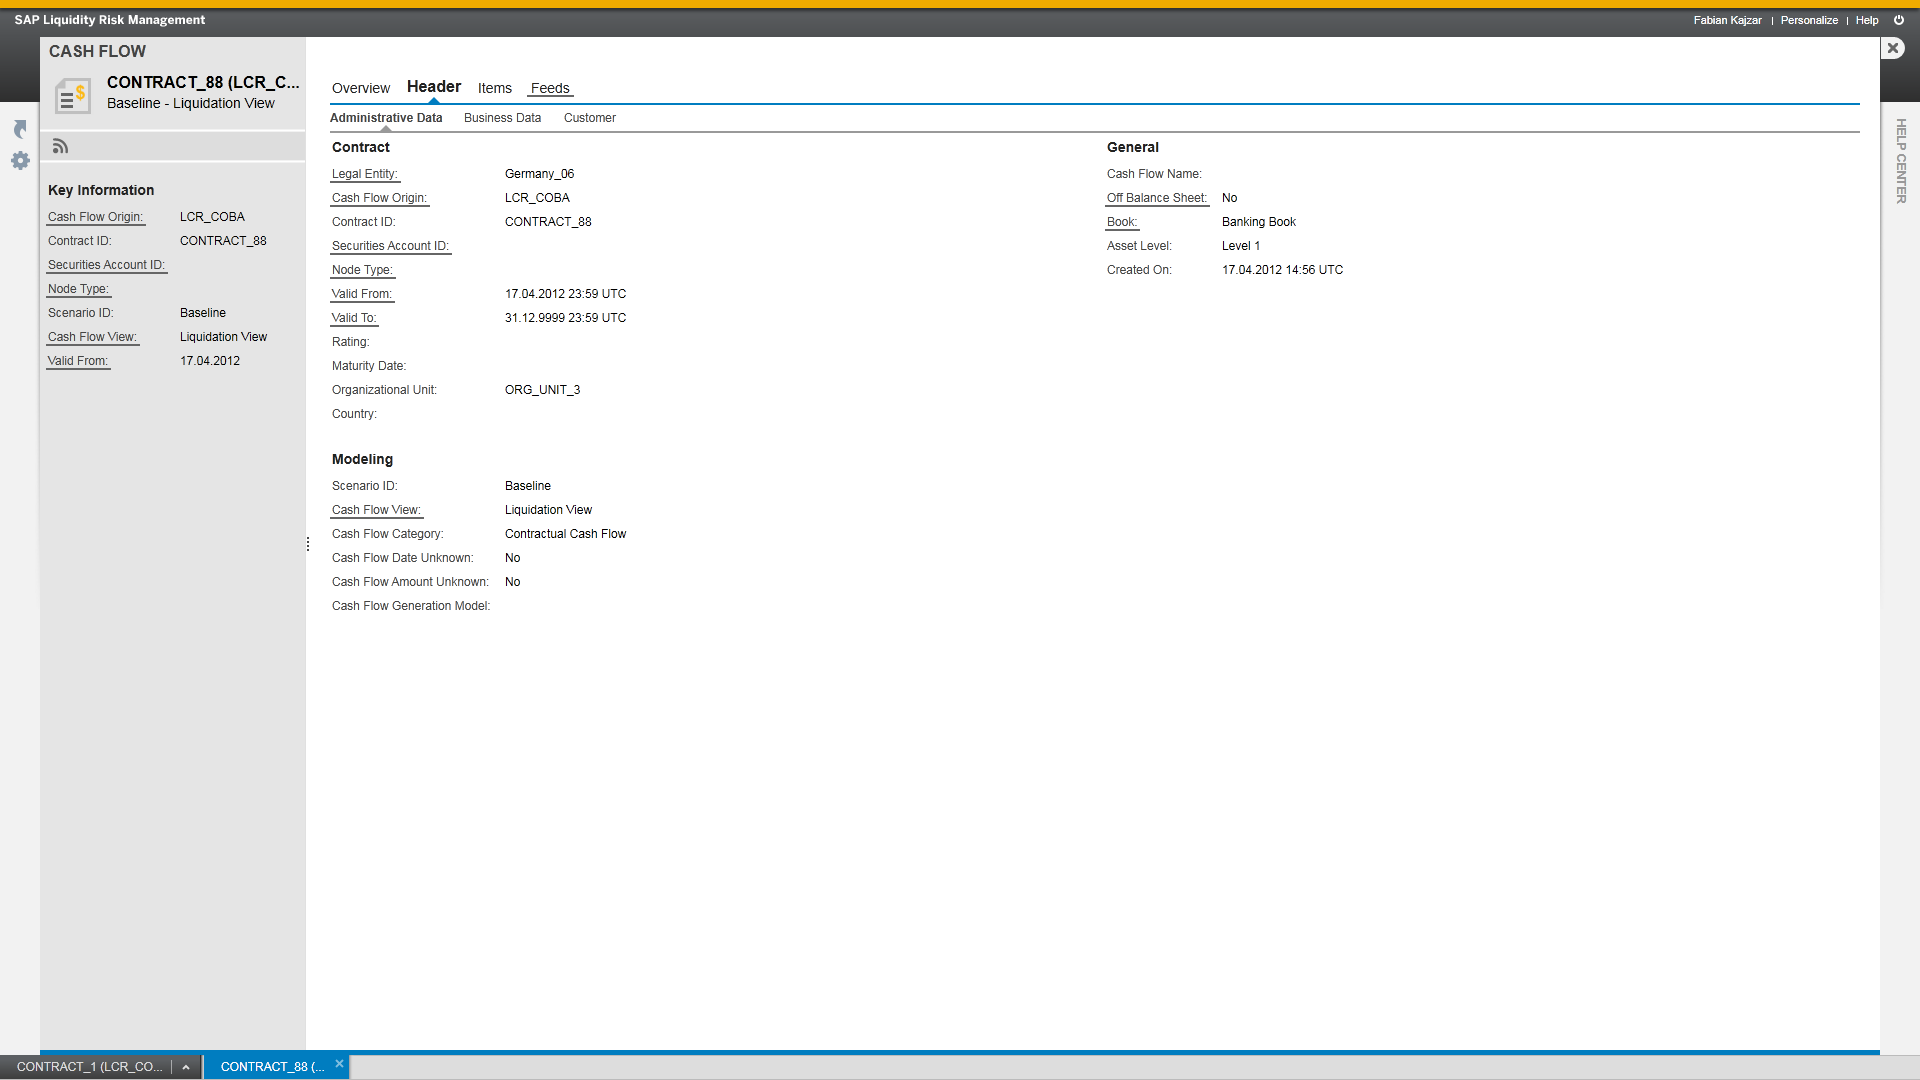
\includegraphics[width=15cm]{images/OberonUI.png}
\caption{Darstellung eines CashFlows-Eintrags mit dem Oberon-Framework\label{fig:oberon}}
\end{figure}

Oberflächen werden mit dem Oberen Framework mit der Programmiersprache C\# und Microsoft Silverlight\footnote{Microsoft Silverlight - http://www.microsoft.com/silverlight/} entwickelt. Silverlight ist eine Technologie von Microsoft, die als Plugin für verschiedene moderne Browser verfügbar ist und die Entwicklung von \gls{glos:ria} unterstützt. Die \gls{glos:ria} stellt dabei die erste Schicht der drei Schichtenarchitektur von Oberon dar. Die weiteren Schichten, Die Anwendungslogik und die Persistenz, werden von NGAP und HANA übernommen.\seFootcite{vgl.}{}{Oberon-A}

Das Oberon Framework ist als Standardframework ausgelegt und versucht, möglichst viele Anforderungen abzudecken um so in vielen Produkten verwendet werden zu können. Allerdings ist es sehr Wahrscheinlich, dass spezielle Anforderungen eines bestimmten Bereichs nicht mit der aktuellen Version des Oberon Frameworks abgedeckt werden können. In diesem Fall müssen eigene Lösungen für die Anforderungen entwickelt werden.\seFootcite{vgl.}{}{Oberon-A}

\subsection{Berechnungskomponente}
Die Berechnungskomponente stellt den wichtigsten Teil des SAP LRM dar. Mit ihr werden alle Berechnungen im Umfeld des Liquiditätsrisikomanagements zentral durchgeführt. Die Berechnung findet auf Basis von Liquiditätsgruppen statt. Mit Hilfe von Liquiditätsgruppen werden sowohl aggregierter Zahlungsstrom als auch Kennzahlen einheitlich berechnet. Liquiditätsgruppen können in Polyhierarchien\footnote{Polyhierarchien sind hierarchische Strukturen, bei der ein Element mehrere übergeordnete Elemente haben kann.} angeordnet werden. Dadurch können Berechnungen modular aufgebaut, wiederverwendet und einfach nachvollzogen werden. Das Abbilden von komplexen Berechnungsvorschriften wird erleichtert.\seFootcite{vgl.}{S.38}{LRM-PPT.12}

Es existieren genau zwei Arten von Liquiditätsgruppen, der Datenbankselektion und der Berechnung. Die Datenbankselektion bildet immer den Ursprung einer Berechnung. Dabei werden einzelne Zahlungsströme von der nach Selektionskriterien selektiert, und nach Bedingungen Zusammengefasst. Selektionskriterien können z.B. der hinterliegende Produkttyp des Zahlungsstroms wie z.B. verzinsliches Wertpapier, oder das entsprechende Finanzraiting, z.B. AAA sein. Gleichzeitig findet eine Währungsumwandlung in eine einheitliche Zielwährung statt. Mehrere Zahlungsströme werden in Abhängigkeit ihrer Fälligkeit in Behältern zusammengefasst. Diese Behälter werden von dem festgelegten Fälligkeitsband definiert.\seFootcite{vgl.}{S.40}{LRM-PPT.12}

Ein Fälligkeitsband ist eine spezielle Einteilung der Zeitachse. Der Grund für die Einführung von Fälligkeitsbändern liegt in der späteren Auswertung der berechneten Werte. Dabei ist für naheliegende Zeiträume, z.B. die nächste Woche, der entsprechende Wert an jedem einzelnen Tag entscheidend. Für den weiteren Horizont, z.B. den Zeitraum zwischen 3 und 5 Jahren, ist nicht jeder einzelne Tag  entscheidend, es reichen aggregierte Werte, z.B. nach Monat oder Jahr. Somit kann in einer Auswertung sowohl die aktuelle Situation begutachtet werden, als auch die langfristige Auswirkungen ohne, dass die Auswertung unübersichtlich wird. Jeder Eintrag entspricht dabei einem Behälter. Die Anzahl und Größe der Behälter ist in einem Fälligkeitsband definiert.[TODO beispiel]\seFootcite{vgl.}{S.44}{LRM-PPT.12}

Neben der Datenbankselektion existiert die Liquiditätsgruppenart Berechnung. Dabei werden aggregierte Zahlungsströme nach verschiedenen Regeln verrechnet. Zur Verfügung stehende unter Anderem Addition, Subtraktion, Multiplikation und Division. Generell hat eine Liquiditätsgruppe genau einen Output-Parameter, eine Berechnungsregel und kann zusätzlich mehrere Input-Parameter besitzen. Die Berechnung innerhalb einer Liquidiätsgruppe kann von szenarioabhängigen Variablen beeinflusst werden. Damit lassen sich z.B. erwartete Kreditausfälle simulieren. Über diese Variablen werden die Szenarien umgesetzt. Mehrere Variablenausprägungen legen ein Szenario fest.\seFootcite{vgl.}{S.39 und S.45}{LRM-PPT.12}

Zur Laufzeit wird die Berechnungskomponente mit 4 Parametern aufgerufen. In dem ersten Parameter werden eine oder mehrere Liquiditätsgruppen festgelegt, von denen später das Ergebnis zurückgeliefert wird. Ein weiterer Parameter legt den Stichtag fest, nach dem die Zahlungsströme ausgewählt werden. Jede Berechnung wird immer auf Basis von einem Fälligkeitsband durchgeführt, welches die Behälter festlegt, in dem die Ergebnisse zusammengefasst werden. Schließlich wird noch eine Zielwährung festgelegt, in die alle Zahlungsströme umgerechnet werden. Das Resultat der Berechnung ist jeweils der Output der festgelegten Liquiditätsgruppen. Zur Berechnung der Gruppen müssen in der Regel im Hintergrund weitere Liquiditätsgruppen berechnet werden, die allerdings nicht als Ergebnis zurückgeliefert werden. Während einer Berechnung werden Ergebnisse von Gruppen, die schon einmal berechnet wurden, zwischengespeichert um Rechenaufwand zu sparen. Die Gruppen, die berechnet werden müssen, können aus der Hierarchie der entsprechenden Liquiditätsgruppe abgelesen werden.\seFootcite{vgl.}{S.44 und S.47}{LRM-PPT.12}

\section{Xcelsius}
\subsection{Funktionen}
Xcelsius ist ein Teil der SAP Business Objects Portfolio. Dabei handelt es sich um Anwendungen, mit denen Daten in einem Unternehmen analysiert und ausgewertet werden können. Xcelsius ist davon ein Tool zur Visualisierung von Daten durch die Erstellung von interaktiven Dashboards.

Dazu bietet es viele Möglichkeiten um Daten visualisieren und interaktiv beeinflussen zu können. Neben 20 Diagrammtypen, darunter unter anderem Linien-, Kreis-, Balken-  und Flächendiagramme stehen Schaltflächen zur Manipulation wie Schieberegler, Optionsfelder und Drehknöpfe zur Verfügung. Zusätzlich können Kartenelemente zur Darstellung von Geoinformationen genutzt werden und Bilder und Texte unterstützend in ein Dashboard eingebunden werden. Viele Komponenten bieten zusätzlich Einstellungsmöglichkeiten, durch die das Aussehen oder das Verhalten an die Anforderungen angepasst werden kann.\seFootcite{vgl.}{S.31f und S.229f}{Egg.09}

Die Daten, auf denen die Visualisierungen in Xcelsius basieren, werden durch die Integration von Microsoft Excel verwaltet. Excel steht dabei in vollem Umfang zur Verfügung, es können also sowohl  Berechnungen, als auch Formatierungen mit Excel durchgeführt werden. Excel wird hierbei als Schnittstelle zwischen der Datenbeschaffung aus verschiedensten Quellen und der eigentlichen Visualisierung genutzt. Alle Daten, die visualisiert werden sollen, werden in das Tabellenkalkulationsblatt von Excel geschrieben und von dort aus ausgelesen. Die Daten können demnach vor der Darstellung in Excel beliebig bearbeitet werden.\seFootcite{vgl.}{S.32 und S.236}{Egg.09}

Die gesamte Erstellung eines Dashboards findet nach dem „What you see is what you get“-Prinzip statt. Der Anwender sieht schon während der Erstellung, wie das Ergebnis aussieht. Durch die Verwendung von Excel und dem Umsetzen des Wysiwyg-Prinzip benötigen Nutzer meist nur eine geringe Einarbeitungszeit und die Bedienung kann als intuitiv beschrieben werden. Besondere Programmiersprachenkenntnisse sind für die Erstellung von Dashboards nicht erforderlich.\seFootcite{vgl.}{S.32 und S.239}{Egg.09}

Die mit Xcelsius erstellten Dashboards werden mit Hilfe der Adobe Flex Technologie dargestellt. Dadurch ist kein extra Server oder gar eine Datenbank notwendig. Es wird nur das Flash-Plugin benötigt. Außerdem muss dafür für die Darstellung keine Netzwerkverbindung zu einem Server oder dem Internet vorhanden sein.  Zusätzlich können Dashboards in verschiedene Formate exportiert werden um sie so in Microsoft PowerPoint-Präsentationen oder auf Internetseiten einzubinden.\seFootcite{vgl.}{S.31f und S.230}{Egg.09}

Als Datenquellen für ein Dashboard stehen mehrere Möglichkeiten zur Verfügung. Zum einen können Daten einfach in das Excel kopiert werden.  Es ist auch möglich, ein SAP Business Warehouse System direkt anzuschließen, oder Daten über Webservices zu beziehen. Hierzu das XML-Format verwendet. Außerdem existieren weitere Möglichkeiten, wodurch Dashboards z.B. untereinander Daten austauschen können.\seFootcite{vgl.}{S.283f}{Egg.09}

\subsection{Bedienungskonzept}
Die Oberfläche von Xcelsius lässt sich in 4 Bereiche Aufteilen. Die Bereiche sind in \vref{fig:xcelsius_ui_aufbau} dargestellt. Der erste Bereich zeigt die Zeichenfläche, also das eigentliche Dashboard an. Durch die Umsetzung des WYSIWYG-Prinzips kann schon während der Erstellung des Dashboards das spätere Ergebnis dargestellt werden. Auf der Zeichenfläche können Komponenten beliebig platziert werden. Alle verfügbaren Komponenten werden in dem Bereich 2 auf der linken Seite nach Kategorien geordnet dargestellt. Um eine Komponente auf der Zeichenfläche zu platzieren, wählt der Nutzer die Komponente aus und platziert sie per Drag\& Drop auf der Zeichenfläche. 

\begin{figure}[h]
\centering
\setlength{\unitlength}{1mm}
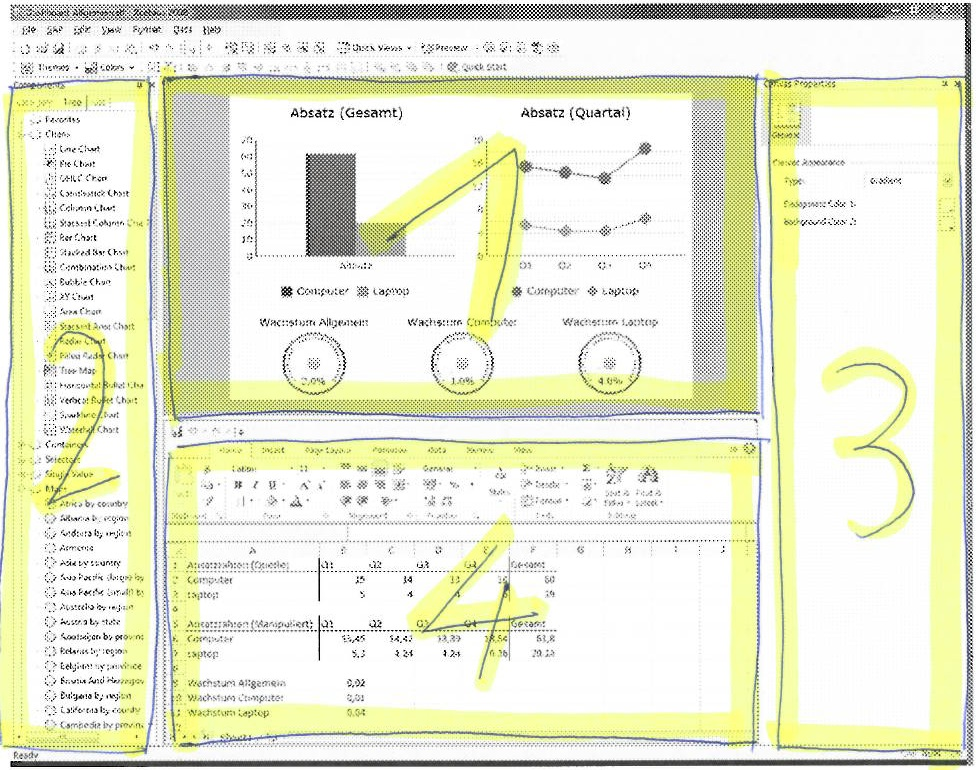
\includegraphics[width=15cm]{images/Xcelsius_UI_Aufbau.jpg}
\caption{[TODO]\label{fig:xcelsius_ui_aufbau}}
\end{figure}

Viele Komponenten bieten Einstellungsmöglichkeiten an, mit denen das Verhalten und das Aussehen der Komponente festgelegt werden kann. Wird eine Komponente auf der Zeichenfläche ausgewählt, werden alle verfügbaren Eigenschaften in Bereich 3 auf der rechten Seite dargestellt. Wichtige Eigenschaften einer Komponente stellen oft die Daten dar, die die Komponenten anzeigen soll. Alle Daten werden in Bereich 4 festgelegt. Dafür steht der volle Funktionsumfang von Microsoft Excel zur Verfügung. Die Verbindung zwischen der Datenhalten (Microsoft Excel in Bereich 4) und der Darstellung (Zeichenfläche in Bereich 1) von Xcelsius erfolgt durch das Referenzieren von Zellen oder Zellbereichen über die Eigenschaften einer Komponente (Bereich 3).\seFootcite{vgl.}{S.229}{Egg.09}

Der generelle Ablauf des Erstellens von Dashboards soll an dem Beispiel der Absatzzahlen von Produkten in \vref{fig:xcelsius_ui_beispiel} verdeutlicht werden: Zunächst werden Daten in das Excel in einen festgelegten Bereich Eingetragen. Dies Daten können entweder fest eingegeben werden, meistens werden sie aber dynamisch über eine Datenquelle, z.B. einen Webservice in den Bereich geschrieben. In dem Beispiel wurden die Absatzzahlen händisch in den Zellbereich 1 eingetragen. Als nächstes können in Excel Berechnungen durchgeführt werden. In dem Beispiel wird die Summe der Absatzzahlen pro Jahr durch eine Excel-Formel berechnet. Um die Interaktivität von Dashboards zu zeigen, soll der Nutzer die Möglichkeit haben, die Auswirkungen von verschiedenen Wachstumsraten interaktiv zu sehen. Dazu werden die veränderten Absatzzahlen (Bereich 2) auf Basis der Quelldaten in Bereich 1 und den Wachstumsdaten in Bereich 3 berechnet.\seFootcite{vgl.}{S.229f}{Egg.09}

\begin{figure}[h]
\centering
\setlength{\unitlength}{1mm}
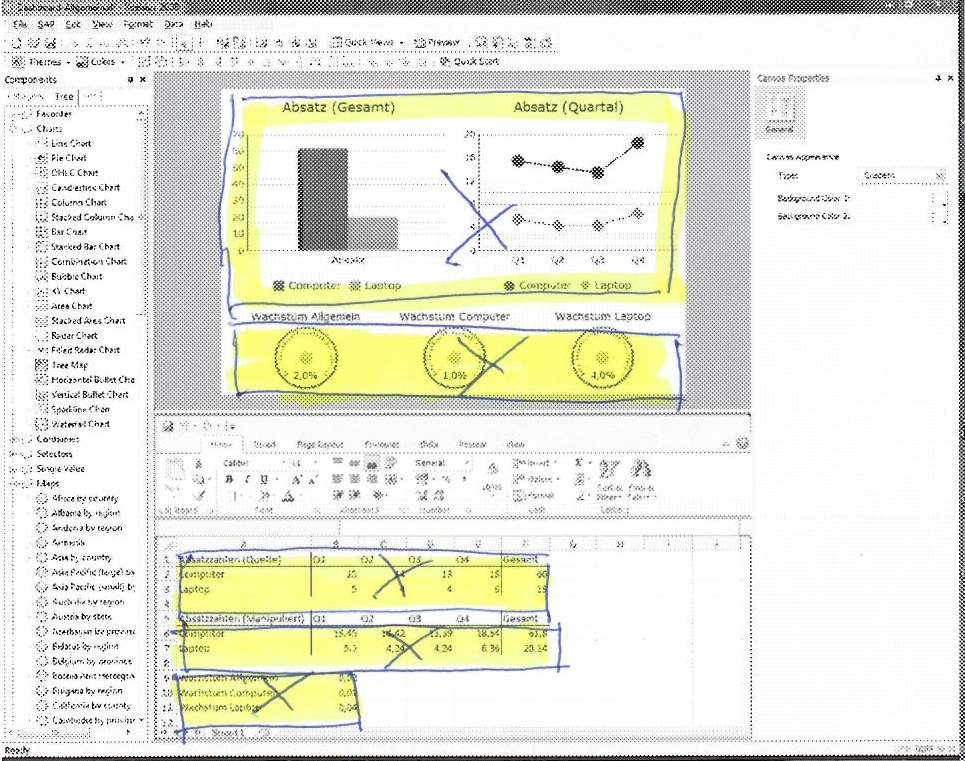
\includegraphics[width=15cm]{images/Xcelsius_UI_Beispiel.jpg}
\caption{[TODO]\label{fig:xcelsius_ui_beispiel}}
\end{figure}

Schließlich werden auf der Zeichenfläche zwei Diagramme festgelegt, die ihre Daten aus Bereich 2 auslesen. Die Wachstumsraten können mit drei Drehknöpfe festgelegt werden. Die Werte der Drehknöpfe sind mit den Zellen in Bereich 3 verknüpft. Dreht der Nutzer an einem Drehknopf, wird der aktualisierte Wert in die Zelle in Bereich 3 geschrieben. Da die Datenquelle der Graphen mit Bezug auf die Wachstumswerte berechnet werden, verändert sich dynamisch die Graphen. Das Prinzip ist schematisch noch einmal in \vref{fig:xcelsius_ablauf_schema} dargestellt. So ist es möglich, mit einfachen Mitteln interaktive Dashboards zu erstellen.\seFootcite{vgl.}{S.237}{Egg.09}

\begin{figure}[h]
\centering
\setlength{\unitlength}{1mm}
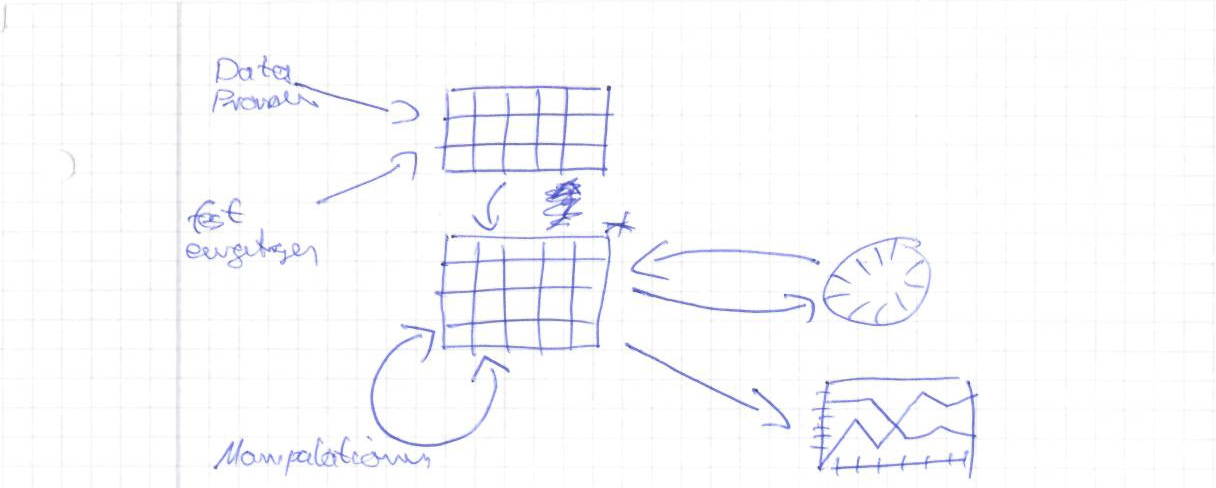
\includegraphics[width=15cm]{images/Xcelsius_UI_Ablauf.jpg}
\caption{[TODO]\label{fig:xcelsius_ablauf_schema}}
\end{figure}

\subsection{Architektur}

Xcelsius basiert auf dem .Net [TODO] Framework von Microsoft und ist in weiten Teilen in C++ geschrieben. Neben C++ wird Action Script und das Adobe Flex Framework für die  Benutzeroberfläche eingesetzt. Die Architektur von Xcelsius ist modular aufgebaut und besteht aus mehreren Teilen. Ein Überblick ist in \vref{fig:xcelsius_architektur} dargestellt.

\begin{figure}[h]
\centering
\setlength{\unitlength}{1mm}
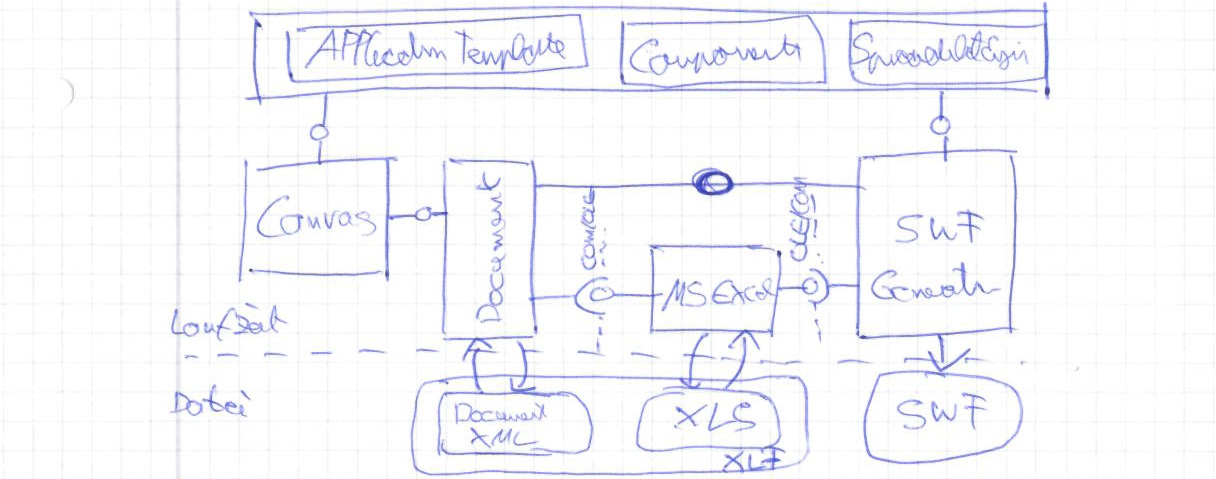
\includegraphics[width=15cm]{images/Xcelsius_Architecture.jpg}
\caption{[TODO]\label{fig:xcelsius_architektur}}
\end{figure}

Das zentrale Element ist das Document. Dabei handelt es sich um ein Objektmodell, das den aktuellen Zustand des Dashboards repräsentiert. Für die Darstellung wird das Canvas verwendet, welches in ActionScript 3 geschrieben ist. Die Canvas-Komponente nutzt dabei mehrere Hilfskomponenten. Dazu gehört das ApplicationTemplate, welches das Grundgerüst von alle Dashboards darstellt und mehreren Components, die die eizelnen Elemente eines Dashboards darstellen. Dies ist auch der Ansatzpunkt für spätere Erweiterungen.

An das Document ist mittels COM/OLE [TODO] Microsoft Excel angebunden. Speichern und Laden eines Dashboards übernimmt die XLF-Komponente. Diese erstellt oder lädt eine Xcelsius File (.xlf), welches intern aus dem Document im XML-Format und einer Exceldatei besteht.

Für den Export des fertigen Dashboards existiert der SWF Generator. Aus dem Document und den Daten und Formeln, die in Microsoft Excel erstellt wurden, wird eine .swf Datei generiert. In dieser werden nun alle Berechnungen, die bis jetzt von Microsoft Excel übernommen wurden, von einer weiteren Hilfsklasse, der Spreadsheet Engine berechnet.\seFootcite{vgl.}{}{Xcelsius-Arch.09}


\subsection{Erweiterungsmöglichkeiten}

Durch die Einstellungsmöglichkeiten der einzelnen Komponenten und die Einbindung des vollen Funktionsumpfang von Microsoft Excel ist Xcelsius von sich aus sehr flexibel. Zusätzlich dazu existiert noch ein SDK [TODO Glos?] mit dem komplett eigene Komponenten erstellt werden können. Dadurch ist es möglich, Xcelsius um nahezu beliebige Funktionen zu erweitern.

Die Erweiterungen, die mit dem SDK programmiert werden können, müssen auf dem Adobe Flex SDK 2.0.1 basieren. Die Programmiersprache ist Action Scritp [TODO Glos]. Es können drei verschiedene Typen von Erweiterungen mit dem SDK entwickelt werden. Dabei handelt es sich um visuelle Komponenten, die später auf dem erstellten Dashboard dargestellt werden, um Datenverbindungen, die nicht auf dem Dashboard angezeigt werden, sondern nur im Hintergrund aktiv sind und in der Regel Daten in das Excel eintragen. Die dritte Möglichkeit ist die Erweiterung der Steuerungslogik von Excel, spielt aber im Rahmen dieser Bachelorarbeit keine Rolle. \footnote{\seCite{vgl.}{S.229}{Egg.09} \seCite{und}{S.3f}{Xcelsius-SDK.08}}

Die visuelle Komponente wiederum besteht aus zwei Teilen, die separat von einander entwickelt werden können. Der erste Teil ist für die Darstellung der Komponente auf dem Zeichenblatt des Dashboards verantwortlich. Der zweite Teil übernimmt die Darstellung der Eigenschaften, die die Komponente bieten soll. Es ist gleichzeitig die Verbindung zwischen Xcelsius und der entwickelten Komponente. Die Logik der Komponente kann je nach Bedarf auf beide Teile verteilt werden. Das Ergebnis der Entwicklung der beiden Teilkomponenten sind zwei kompilierte .swf Dateien [TODO !?]. Diese Dateien, in Verbindung mit Informationen zu der Komponente, wie z.B. Name, Version, Typ und Entwickler werden mit dem Xcelsius SDK zu einem Xcelsius Plugin zusammengefügt. Dieses kann dann in Xcelsius importiert und die Komponenten so genutzt werden.\footnote{\seCite{vgl.}{S.283f}{Egg.09} \seCite{und}{S.6}{Xcelsius-SDK.08}} Den Vorgang zeigt \vref{fig:xcelsius_plugin}.

\begin{figure}[h]
\centering
\setlength{\unitlength}{1mm}
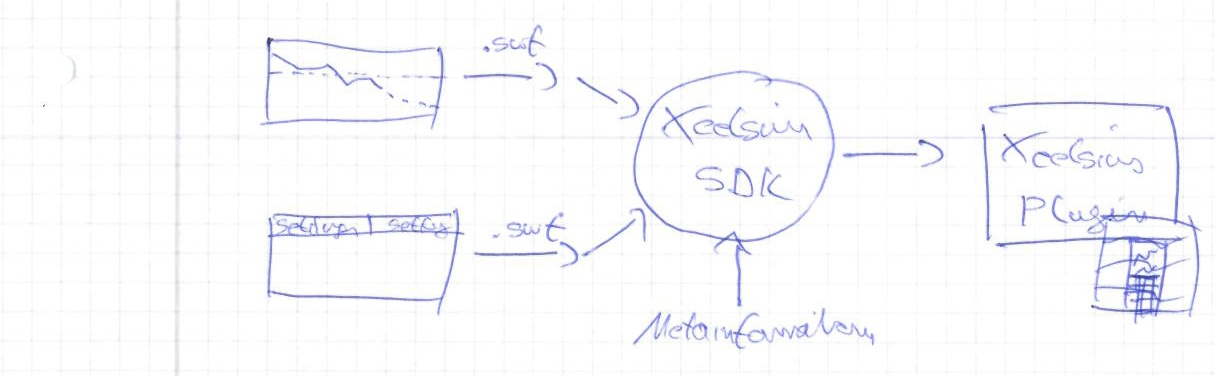
\includegraphics[width=15cm]{images/Xcelsius_Plugin_Allgemein.jpg}
\caption{[TODO]\label{fig:xcelsius_plugin}}
\end{figure}

\section{Zusammenfassung}

\chapter{Spezifikation}
\section{Einleitung}
\section{Ausgangssituation}
\section{Zielsetzung}
\section{Anforderungen}
\section{Zusammenfassung}

\chapter{Umsetzungsmöglichkeiten}
\section{Einleitung}
\section{WebService}
\section{Zusammenfassung}

\chapter{Umsetzung}
\section{Einleitung}
\section{Analyse}
\section{Entwurf}
\section{Implementierung}
\section{Zusammenfassung}

\chapter{Evaluation}
\section{Einleitung}
\section{Möglichkeiten}
\section{Vergleich}
\section{Performance}
\section{Zusammenfassung}

\chapter{Zusammenfassung}


% -------------------------------------------------------------------------------------
% Anhang der Arbeit
% -------------------------------------------------------------------------------------
\seAppendix{}

\pagenumbering{Roman}
\setcounter{page}{8}

\chapter{Anhang}

Inhalt des Anhangs

% -------------------------------------------------------------------------------------
%  Erzeugung eines Glossars
% -------------------------------------------------------------------------------------
\newpage
\sePrintGlossary{}

% -------------------------------------------------------------------------------------
% Literaturverzeichnisses
% -------------------------------------------------------------------------------------
\sePrintBibliography{}


% Sammelwerke, die in der Grundform vorkommen sollten!
%\nocite{Bar.08}
%\nocite{Rom.10}
%\nocite{Zer.10}
%\nocite{Hof.11}
%\nocite{Eve.08}

\bibliographystyle{sty/bibliothek-style}
\seBibliography{literatur}

% -------------------------------------------------------------------------------------
% Erzeugung der ehrenw\"ortlichen Erkl\"arung
% -------------------------------------------------------------------------------------
\seEhrenwoertlicheErklaerung{}

\end{document}
